\documentclass[10pt,c]{beamer}

\usepackage[T1]{fontenc}
\usepackage[utf8]{inputenc}
\usepackage{graphicx}
\usepackage{multirow}


%%%%%%%%%%%%%%%%%%%%%%%%%%%%%%%%%%%%%%%%%%%%%%%%%%%%%%%%%%%%%%%%%%%%%%%%%%%%%%%%
%%%                               80 COLONNES                                %%%
%%%%%%%%%%%%%%%%%%%%%%%%%%%%%%%%%%%%%%%%%%%%%%%%%%%%%%%%%%%%%%%%%%%%%%%%%%%%%%%%

%%% THÈME DE LA PRÉSENTATION
\usetheme{JuanLesPins}  %% Warsaw

%%% ÉLÉMENTS DE TITRE
\title{Using Cooja for WSN Simulations: Some New Uses and Limits}
\author{Kévin Roussel \and Ye-Qiong Song \and Olivier Zendra}
\institute{INRIA Nancy Grand-Est~---
           LORIA UMR~7503~--- Université de Lorraine}
\date{EWSN'2016 NextMote workshop\\
      \textit{15 February 2016}}
\titlegraphic{
    \vspace{0.25cm}%
    
\includegraphics[height=1cm]{logo_inria_en.png}%
    \hspace{2cm}~%
    
\includegraphics[height=1cm]{logo_loria.png}%
    \hspace{2cm}~%
    
\includegraphics[height=1cm]{logo_ul.png}%
}

%%%%%%%%%%%%%%%%%%%%%%%%%%%%%%%%%%%%%%%%%%%%%%%%%%%%%%%%%%%%%%%%%%%%%%%%%%%%%%%%
%%%                               80 COLONNES                                %%%
%%%%%%%%%%%%%%%%%%%%%%%%%%%%%%%%%%%%%%%%%%%%%%%%%%%%%%%%%%%%%%%%%%%%%%%%%%%%%%%%

%%% COMMANDES UTILES AU COURS DU CORPS DE TEXTE

\renewcommand{\emph}[1]{\textbf{\textit{#1}}}
\newcommand{\nom}[1]{\textbf{#1}}
\newcommand{\tblcaption}[1]{\textbf{\textsl{\small#1}}\vspace{0.1cm}}

\setbeamertemplate{itemize item}[square]
\setbeamertemplate{itemize subitem}[triangle]
\setbeamertemplate{itemize subsubitem}[circle]
\setbeamertemplate{bibliography item}{\insertbiblabel}
% Ajout des numéros de transparents à la barre de navigation en bas à droite
\setbeamercolor{footline}{fg=darkgray}
\setbeamerfont{footline}{series=\bfseries,size=\scriptsize}
\addtobeamertemplate{navigation symbols}{}{%
    \usebeamerfont{footline}%
    \usebeamercolor[fg]{footline}%
    \hspace{1.5em}%
    \insertframenumber~/ \insertpresentationendpage
}

%%%%%%%%%%%%%%%%%%%%%%%%%%%%%%%%%%%%%%%%%%%%%%%%%%%%%%%%%%%%%%%%%%%%%%%%%%%%%%%%
%%%                               80 COLONNES                                %%%
%%%%%%%%%%%%%%%%%%%%%%%%%%%%%%%%%%%%%%%%%%%%%%%%%%%%%%%%%%%%%%%%%%%%%%%%%%%%%%%%

%%% DÉBUT DE LA PRÉSENTATION
\begin{document}

%%% TITRE
\begin{frame}
\titlepage
\end{frame}

%%% SOMMAIRE GÉNÉRAL

\begin{frame}
\frametitle{Contents}
\tableofcontents
\end{frame}

%%%%%%%%%%%%%%%%%%%%%%%%%%%%%%%%%%%%%%%%%%%%%%%%%%%%%%%%%%%%%%%%%%%%%%%%%%%%%

\section{Introduction}

\begin{frame}
\frametitle{Introduction I}
\begin{block}{To develop and test large, ambitious WSN-based projects}
$\rightarrow$ need of powerful and accurate simulation/emulation tools
\end{block}
\begin{block}{Many such simulation/emulation tools for WSNs exist:}
\begin{itemize}
\item OpenSim (from OpenWSN project)
\item TOSSIM (from TinyOS project)
\item Cooja (from Contiki OS project)
\end{itemize}
\end{block}
\begin{exampleblock}{This work focuses on the latter framework: \nom{Cooja}}
$\rightarrow$ (one of) the most used WSN simulation/emulation tool
\end{exampleblock}
\end{frame}

\begin{frame}
\frametitle{Introduction II}
\begin{block}{Contributions of our work: we will focus on\ldots}
\begin{enumerate}
\item the ability---\emph{actually tested and used}---to use the Cooja
framework to simulate/emulate systems not related to Contiki OS
\item the inaccuracies in time-related results we discovered while using
Cooja\footnote{Note we always used the Cooja version provided with
Contiki release 2.7} to perform our own simulations to test our own
WSN-related projects
\item the possible consequences of these inaccuracies in the literature
published in the WSN domain
\end{enumerate}
\end{block}
\end{frame}

%%%%%%%%%%%%%%%%%%%%%%%%%%%%%%%%%%%%%%%%%%%%%%%%%%%%%%%%%%%%%%%%%%%%%%%%%%%%%

\section{Cooja and MSPSim}

\begin{frame}
\vspace{-0.5cm}
\frametitle{The Cooja framework and its emulators}
\center{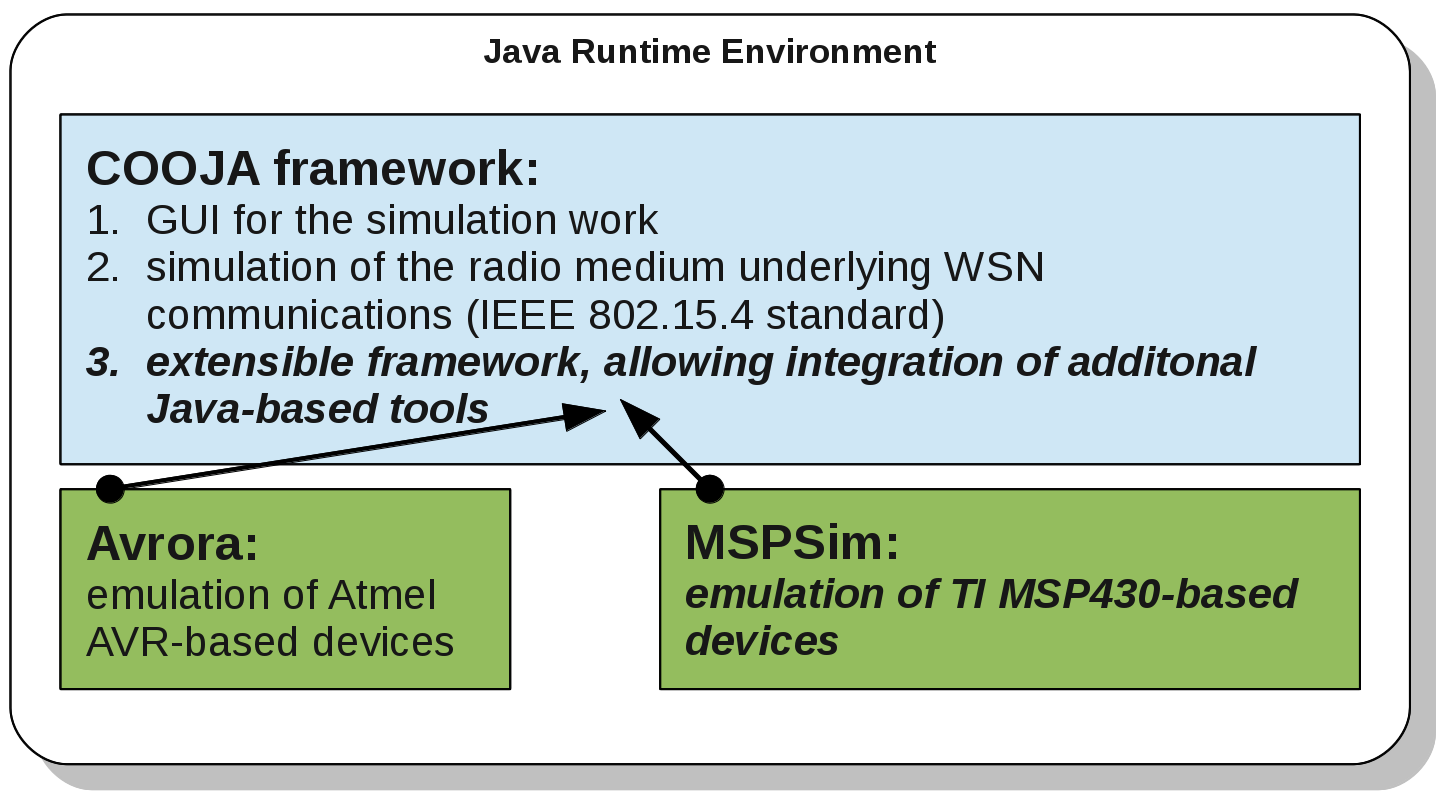
\includegraphics[width=10cm]{CoojaFramework.png}}

\vspace{0.25cm}
\begin{block}{}
\emph{The present work focuses on Cooja and the MSPSim emulator only}
\end{block}
\end{frame}

%%%%%%%%%%%%%%%%%%%%%%%%%%%%%%%%%%%%%%%%%%%%%%%%%%%%%%%%%%%%%%%%%%%%%%%%%%%%%

\section{Using Cooja and MSPSim: Not Only for Contiki!}

\begin{frame}
\frametitle{Using Cooja and MSPSim with any WSN system\ldots \\
            (or even without)}
\begin{block}{What do Cooja's embedded emulators run?}
\small
The Contiki build system produces standard (ELF format) executables \\
$\rightarrow$ the Cooja embedded emulators are designed to run such
standard executables
\end{block}
\begin{exampleblock}{What does it mean?}
\small
\emph{Any system producing such standard ELF executables (besides Contiki
OS itself) will run on virtual motes emulated with the Cooja framework}

We tested this with MSPSim, using:
\begin{itemize}
\item applications based on RIOT OS
\item ``bare-metal'' applications
\end{itemize}

Any other OS using \texttt{msp430-gcc} as its compiler (e.g.: TinyOS)
should run fine on Cooja/MSPSim: a simple trick on executables' file
extension is enough
\end{exampleblock}
\end{frame}

%%%%%%%%%%%%%%%%%%%%%%%%%%%%%%%%%%%%%%%%%%%%%%%%%%%%%%%%%%%%%%%%%%%%%%%%%%%%%

\section{Timing Inaccuracy Problem in MSPSim}

\subsection{The Setup}

\begin{frame}
\frametitle{Timing Inaccuracy Problem in MSPSim: Setup}
\begin{alertblock}{What did we discover during our experiments?}
\begin{itemize}
\item unexplained delays during simulations/emulations of packet
transmissions (TX), not observed on real hardware
\item the differences appear on one peculiar operation: \emph{when loading
the TX buffer of the CC2420 radio transceiver}
%(common to both our hardware platforms: Sky/TelosB and Zolertia Z1 motes)
\end{itemize}
\end{alertblock}
\begin{block}{What did we do to investigate that problem?}
\begin{itemize}
\item we wrote a simple test program, which only sends data packets of
various sizes (resp. 30, 60 and 110 bytes of MAC payload)
%to which a MAC layer-related overhead of 11 bytes is always added
\item we tried this program on various configurations:
  \begin{itemize}
  \item two different hardware platforms: Sky/TelosB and Zolertia Z1 motes
  \item two different WSN OS: Contiki and RIOT OS
  \end{itemize}
\end{itemize}
\end{block}
\end{frame}

\subsection{The Results}

\begin{frame}
\frametitle{Timing Inaccuracy Problem in MSPSim: Results I}
\begin{center}
\vspace{-0.9cm}
\small
\[
\mbox{\textbf{Inaccuracy}}
   = \frac{\mbox{Simulated delay} - \mbox{Actual Hardware test delay}}
          {\mbox{Actual Hardware test delay}}
\]

\vspace{0.1cm}

\tblcaption{\small Observed TX buffer loading delay inaccuracies of MSPSim
            emulation \\ versus tests on actual hardware}
\begin{tabular}{|l|l|r|r|}
\hline
\textbf{HW platform} & \textbf{OS} & \textbf{Payload size}
                     & \textbf{Inaccuracy} \\
\hline
SkyMote/TelosB & Contiki &  30 bytes &  11\% \\
SkyMote/TelosB & Contiki &  60 bytes &  15\% \\
SkyMote/TelosB & Contiki & 110 bytes &  13\% \\
\hline
SkyMote/TelosB & RIOT OS &  30 bytes &  15\% \\
SkyMote/TelosB & RIOT OS &  60 bytes &  16\% \\
SkyMote/TelosB & RIOT OS & 110 bytes &  18\% \\
\hline
Zolertia Z1    & Contiki &  30 bytes & 122\% \\
Zolertia Z1    & Contiki &  60 bytes & 114\% \\
Zolertia Z1    & Contiki & 110 bytes &  95\% \\
\hline
Zolertia Z1    & RIOT OS &  30 bytes & 184\% \\
Zolertia Z1    & RIOT OS &  60 bytes & 185\% \\
Zolertia Z1    & RIOT OS & 110 bytes & 181\% \\
\hline
\end{tabular}
\end{center}
\end{frame}

\begin{frame}
\frametitle{Timing Inaccuracy Problem in MSPSim: Results I}
\begin{block}{What do our tests show?}
\begin{itemize}
\item the inaccuracy problem is mainly influenced by the emulated hardware
platform
  \begin{itemize}
  \item \emph{on Zolertia Z1 motes, timing inaccuracies are catastrophic:
  delays are overestimated by amounts from 95\% to 185\%}
  \item on Sky/TelosB motes, timing inaccuracies are much less important:
  delays are under- or overestimated by amounts up to 18\%
  \end{itemize}
\item the used OS has much less influence on the problem: results tend
to be more accurate on Contiki than on RIOT OS
\item the size of transmitted packets doesn't seem to have any
significative impact on this problem
\end{itemize}
\end{block}
\end{frame}

\begin{frame}
\frametitle{Timing Inaccuracy Problem in MSPSim: Results II}
\begin{center}
\vspace{-0.4cm}
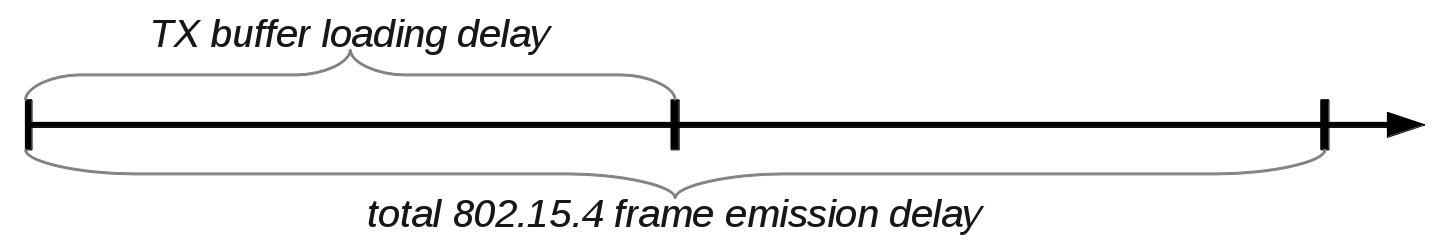
\includegraphics[width=7.5cm]{Delays.png}
\vspace{0.1cm}

\tblcaption{\small Relative weight of TX buffer loading
            in packet transmission delays}
\small
\begin{tabular}{|l|l|r|r|}
\hline
\multirow{2}{2.5cm}{\textbf{HW platform}}
 & \multirow{2}{1cm}{\textbf{OS}}
  & \multirow{2}{2cm}{\textbf{Payload size}}
     & \multicolumn{1}{|c|}{\textbf{\underline{Loading delay}}} \\
 & & & \multicolumn{1}{|c|}{\textbf{Total delay}} \\
\hline
SkyMote/TelosB & Contiki &  30 bytes & 13\% \\
SkyMote/TelosB & Contiki &  60 bytes & 13\% \\
SkyMote/TelosB & Contiki & 110 bytes & 12\% \\
\hline
SkyMote/TelosB & RIOT OS &  30 bytes & 57\% \\
SkyMote/TelosB & RIOT OS &  60 bytes & 53\% \\
SkyMote/TelosB & RIOT OS & 110 bytes & 51\% \\
\hline
Zolertia Z1    & Contiki &  30 bytes & 10\% \\
Zolertia Z1    & Contiki &  60 bytes & 11\% \\
Zolertia Z1    & Contiki & 110 bytes & 10\% \\
\hline
Zolertia Z1    & RIOT OS &  30 bytes & 52\% \\
Zolertia Z1    & RIOT OS &  60 bytes & 48\% \\
Zolertia Z1    & RIOT OS & 110 bytes & 46\% \\
\hline
\end{tabular}
\end{center}
\end{frame}

\begin{frame}
\frametitle{Timing Inaccuracy Problem in MSPSim: Results II}
\begin{block}{What do our tests show \textit{(bis)}?}
\emph{The TX buffer loading operation weight in the whole packet
transmission time is anything but negligible:}

This TX buffer loading operation amounts to about half of the total
packet transmission delay under RIOT OS (much less on Contiki,
where it represents 10\% to 13\%) \\
$\rightarrow$ \textit{This is probably due to the way these OSes do manage
the SPI bus that links the MCU to the radio transceiver on a mote:
\begin{itemize}
\item ``fast mode'' (sending burst of bytes) for Contiki OS
\item ``safe mode'' (checking every byte sent) for RIOT OS
\end{itemize}
}
\end{block}
\end{frame}

\subsection{Discussion}

\begin{frame}
\frametitle{Timing Inaccuracy Problem in MSPSim: Discussion}
\begin{alertblock}{What can we deduce from these results?}
\begin{itemize}
\item \emph{Cooja/MSPSim simulations/emulations do not provide accurate
enough timing-related results}, especially on Zolertia Z1 motes \\
$\rightarrow$ with this inaccuracy issue, \emph{the simulations/emulations
made with this framework cannot be used for timing evaluation purposes
of WSN-based projects}
\item since the hardware seems to be the main factor influencing this
problem, we suppose its cause is---at least partially---linked to wrong
timing calibrations for microcontrollers' emulation 
%\\ {\small (Sky/TelosB microcontroller emulation being visibly much more
%accurate than Zolertia Z1's)}
\end{itemize}
\end{alertblock}
\end{frame}

%%%%%%%%%%%%%%%%%%%%%%%%%%%%%%%%%%%%%%%%%%%%%%%%%%%%%%%%%%%%%%%%%%%%%%%%%%%%%

\section{Consequences}

\begin{frame}
\vspace{-0.25cm}
\frametitle{Consequences on WSN Literature}
\begin{block}{What did we find?}
\begin{itemize}
\item many recent publications rely on Cooja/MSPSim to perform, directly
or indirectly, time-related performance evaluations of their WSN-based
projects
\cite{Constrain-Routing-Trees-2014} \cite{DINAS-2014}
\cite{Efficient-Distrib-Svc-Discovery-2014} \cite{IETF-Routing-WSN-2014}
\cite{TinySDN-2014} \cite{Trickle-L2-2014}
\cite{Visual-Sensor-Networks-2014} \cite{Key-Mgmt-2015}
%(fortunately, most of them use the relatively less impacted Sky/TelosB
%hardware platform)
\item most of these publications are focused on higher layers of WSN
network stacks, like routing protocols 
\cite{Constrain-Routing-Trees-2014}
\cite{IETF-Routing-WSN-2014} \cite{Trickle-L2-2014}
or application-level projects
\cite{DINAS-2014} \cite{Efficient-Distrib-Svc-Discovery-2014}
\cite{Visual-Sensor-Networks-2014} \cite{Key-Mgmt-2015} \\
$\rightarrow$ \emph{their authors may probably be unaware of this problem,}
since they are not focused on low-level details
\end{itemize}
\end{block}
\vspace{-0.25cm}
\begin{alertblock}{What does that mean?}
Many WSN studies rely (at least partially) on Cooja/MSPSim to evaluate
their time-related performances \\
$\rightarrow$ \emph{This inaccuracy problem could make their results
unreliable, and thus put their conclusions in jeopardy!}
\end{alertblock}
\end{frame}

%%%%%%%%%%%%%%%%%%%%%%%%%%%%%%%%%%%%%%%%%%%%%%%%%%%%%%%%%%%%%%%%%%%%%%%%%%%%%

\section{Conclusions}

\begin{frame}
\frametitle{Conclusions I}
\begin{block}{Our contributions:}
\begin{enumerate}
\item we showed that \emph{the Cooja framework is not limited to simulations
of systems running Contiki OS, but can run any program designed for the
emulated architectures} (especially MSP430, thanks to MSPSim)
\item we showed that \emph{the MSPSim emulation---at least for the version
provided with Contiki release 2.7---suffers from a serious timing inaccuracy
issue;} we described the extent of the problem, and provided serious clues
about its cause(s)
\item we briefly enumerated a (non-exhaustive) \emph{list of recent
publications, showing the magnitude of the negative impact}
this problem can cause
\end{enumerate}
\end{block}
\end{frame}

\begin{frame}
\frametitle{Conclusions II}
\begin{alertblock}{In summary:}
Until a fix is made and published to correct this issue in MSPSim,
\emph{we think that all works based on Cooja/MSPSim simulations to evaluate
WSN projects for timing matters should be checked (even partially) by tests
on actual hardware}
\end{alertblock}
\begin{exampleblock}{How to test the accuracy of your own works?}
We provided the source of our test programs (for Contiki and RIOT OS)
on a public GitHub repository:
\center{\texttt{https://github.com/rousselk/tim-inacc-tst-prg}}
\end{exampleblock}
\end{frame}

\begin{frame}
\frametitle{Conclusions III}
\begin{exampleblock}{Strengths of Cooja/MSPSim:}
\begin{itemize}
\item the many publications in the domain of WSNs, especially very recent
ones, including Cooja/MSPSim simulations, is a testimony of the usefulness
of such an emulation framework (especially to test large WSNs, which is
often difficult and expensive to with actual hardware) \\
$\rightarrow$ \emph{That's why we strongly believe fixing Cooja/MSPSim
is really important, and hope for such a fix to appear soon}
\item while the issue described can impair the use of Cooja/MSPSim as
a performance evaluation tool, \emph{it does not affect its other
valuable uses, like the ability to develop and debug WSN-related
software much more easily thanks to its emulation features}
\end{itemize}
\end{exampleblock}
\end{frame}

%%%%%%%%%%%%%%%%%%%%%%%%%%%%%%%%%%%%%%%%%%%%%%%%%%%%%%%%%%%%%%%%%%%%%%%%%%%%%

\section{}

\begin{frame}[b]
\frametitle{Thanks for Your Attention}
\begin{block}{}
\center{\textbf{\Large Any questions?}}
\end{block}
\vspace{1.25cm}
\begin{columns}[c]
\begin{column}{8cm}
\begin{block}{\small Acknowledgements (Funding)}
\small
This work has been funded by the French national PIA
\footnote{\scriptsize\textsl{PIA~: \guillemotleft~Programme
d'investissement d'avenir~\guillemotright}}
\textbf{LAR} (\textit{``Living Assistant Robot''}).
\end{block}
\end{column}
\end{columns}
\vspace{0.3cm}
\end{frame}

%%%%%%%%%%%%%%%%%%%%%%%%%%%%%%%%%%%%%%%%%%%%%%%%%%%%%%%%%%%%%%%%%%%%%%%%%%%%%
%%%                                 ANNEXE                                %%%
%%%%%%%%%%%%%%%%%%%%%%%%%%%%%%%%%%%%%%%%%%%%%%%%%%%%%%%%%%%%%%%%%%%%%%%%%%%%%

\appendix

\section{References}

\setbeamertemplate{navigation symbols}[default]{}

\begin{frame}[t]
\frametitle{References}
\tiny
\bibliographystyle{unsrt}
\bibliography{TimingInacc}
\end{frame}


%%%%%%%%%%%%%%%%%%%%%%%%%%%%%%%%%%%%%%%%%%%%%%%%%%%%%%%%%%%%%%%%%%%%%%%%%%%%%%%%
%%%                               80 COLONNES                                %%%
%%%%%%%%%%%%%%%%%%%%%%%%%%%%%%%%%%%%%%%%%%%%%%%%%%%%%%%%%%%%%%%%%%%%%%%%%%%%%%%%


%%% FIN DE LA PRÉSENTATION
\end{document}


